\documentclass[11pt,a4paper]{article}

\usepackage{fontspec}
\setmainfont{Liberation Serif}
\setsansfont{Liberation Sans}
\setmonofont{Liberation Mono}

\usepackage[english]{babel}
\usepackage[margin=2.2cm,top=2.5cm,bottom=2.5cm,headheight=14pt]{geometry}
\usepackage{amsmath,amssymb}
\usepackage{booktabs}
\usepackage{longtable}
\usepackage{array}
\usepackage{colortbl}
\usepackage{fancyhdr}
\usepackage{tcolorbox}
\tcbuselibrary{breakable}
\usepackage{tikz}
\usetikzlibrary{shapes.geometric,arrows.meta,positioning,calc}
\usepackage{hyperref}

% Color Definitions
\definecolor{sovietred}{RGB}{178,34,34}
\definecolor{techblue}{RGB}{24,76,120}
\definecolor{darkslate}{RGB}{44,62,80}
\definecolor{codebg}{RGB}{245,247,250}
\definecolor{tableheader}{RGB}{230,238,248}
\definecolor{rowalt}{RGB}{248,250,252}

\hypersetup{
    colorlinks=true,
    linkcolor=techblue,
    citecolor=sovietred,
    urlcolor=techblue,
    pdftitle={Elektronika MK-56: Technical Reference Manual},
    pdfauthor={Retrocomputing Engineering}
}

% Headers and Footers
\pagestyle{fancy}
\fancyhf{}
\fancyhead[L]{\small\textcolor{darkslate}{\textbf{Elektronika MK-56} (\textit{Электроника МК-56})}}
\fancyhead[R]{\small\textcolor{darkslate}{Technical Reference \& Microarchitecture}}
\fancyfoot[C]{\thepage}
\renewcommand{\headrulewidth}{0.4pt}
\renewcommand{\footrulewidth}{0pt}

% Box Environments for Technical Notes and Warnings
\newtcolorbox{techbox}[2][]{
    colback=white,
    colframe=techblue,
    arc=1.5mm,
    fonttitle=\bfseries\sffamily,
    title=#2,
    coltitle=white,
    top=3mm,bottom=3mm,left=4mm,right=4mm,
    #1
}

\newtcolorbox{warnbox}[2][]{
    colback=white,
    colframe=sovietred,
    arc=1.5mm,
    fonttitle=\bfseries\sffamily,
    title=#2,
    coltitle=white,
    top=3mm,bottom=3mm,left=4mm,right=4mm,
    #1
}

\begin{document}

\begin{titlepage}
    \centering
    \vspace*{1.5cm}
    
    {\Huge\bfseries\textcolor{darkslate}{Elektronika MK-56}}\\[0.4cm]
    {\LARGE\textbf{\textit{Электроника МК-56}}}\\[1cm]
    
    {\Large\textcolor{techblue}{\textbf{Technical Reference \& Microarchitecture Manual}}}\\[0.3cm]
    {\large Formal Hardware Specification, RPN Stack, Instruction Set, and Flow Control}\\[1.5cm]
    
    \begin{tcolorbox}[colback=codebg,colframe=darkslate,width=0.88\textwidth,arc=2mm]
    \centering\small\sffamily
    \textbf{Normative Reference for Retrocomputing Software Engineering:}\\
    Compilers, Assemblers, Disassemblers, Emulators, and Virtual Machines
    \end{tcolorbox}
    
    \vspace{2cm}
    
    \begin{tabular}{ll}
        \textbf{Computing Family:}      & USSR B3-34 / MK-54 / MK-56 / MK-61 \\
        \textbf{CPU Architecture:}      & K145 PMOS LSI Integrated Circuit Series \\
        \textbf{Computational Model:}   & Reverse Polish Notation (\textit{ПОЛИЗ}) \\
        \textbf{Memory Capacity:}       & 98 program steps, 14 floating-point registers \\
        \textbf{Publication Date:}      & October 2026 \\
    \end{tabular}

    \vfill
    {\small Based on the official USSR factory technical instruction manual (\textit{Инструкция по эксплуатации})\\
    Technical translation, microarchitectural analysis, and typesetting in \LaTeX.}
\end{titlepage}

\tableofcontents
\newpage

\section{Architecture and Stack}

\subsection{Historical Context and Core Circuitry}
The \textbf{Elektronika MK-56} (\textit{Электроника МК-56}) is the desktop mains-powered variant ($220\text{ V AC},\; 50\text{ Hz}$) of the second-generation programmable calculator family manufactured in the USSR. It shares microarchitecture, binary instruction set encoding, execution timing, and cycle dynamics with the handheld models \textbf{Elektronika B3-34} (\textit{Электроника Б3-34}) and \textbf{Elektronika MK-54} (\textit{Электроника МК-54}).

The computational core is constructed around high-density PMOS LSI integrated circuits from the \textbf{K145 series} (\textit{серия К145}):
\begin{itemize}
    \item \textbf{D4 (\textit{К145ИК1302} / K145IK1302):} Main control microcomputer, sequencer, and keyboard decoder. Manages instruction fetch-decode-execute cycles, keypad scanning, VFD refresh routines, and program counter (PC) addressing.
    \item \textbf{D5 (\textit{К145ИК1303} / K145IK1303):} Arithmetic and transcendent function coprocessor. Implements CORDIC micro-algorithms and series expansions for trigonometric, logarithmic, and exponential operations.
    \item \textbf{D6 and D7 (\textit{К145ИР2} / K145IR2):} Dynamic 1008-bit serial shift-register delay lines providing circular storage for the 14 addressable data registers, the 4 operational stack levels, and the subroutine return stack.
    \item \textbf{D8 (\textit{К145АП1} / K145AP1):} Multi-phase clock generator and dynamic timing pulse driver for the PMOS circuitry.
    \item \textbf{D1, D2, D3 (\textit{К161ПП1} / \textit{К161КН1} / K161 series):} High-voltage driver ICs switching phosphor anodes and grid control lines for the vacuum fluorescent display.
\end{itemize}

\subsection{Numeric Format and Vacuum Fluorescent Display (VFD)}
The calculator is equipped with a green-teal 12-digit vacuum fluorescent display (VFD, in Russian: \textit{вакуумно-люминесцентный индикатор}):
\begin{itemize}
    \item \textbf{Mantissa:} 8 decimal significant digits plus 1 sign position.
    \item \textbf{Exponent:} 2 decimal digits plus 1 exponent sign position.
    \item \textbf{Dynamic Representation Range:}
    \[
    \pm 1 \times 10^{-99} \le |x| \le 9.9999999 \times 10^{99}
    \]
    \item \textbf{Fixed-Point vs. Scientific Display Modes:}
    \begin{itemize}
        \item Values within $[10^{-7}, 10^8 - 1]$ automatically display in standard fixed-point decimal notation with the decimal point located at the corresponding place value.
        \item Values outside this range, or upon manual entry via the \texttt{ВП} key (\textit{Ввод Порядка} -- Enter Exponent), transition to scientific floating-point notation:
        \[
        \pm M.MMMMMMM \quad \pm EE
        \]
    \end{itemize}
    \item \textbf{Error Conditions and Overflow:} Arithmetic singularities (division by zero, square root of negative values, non-positive logarithms) or exponent overflow ($> +99$) cause the sequencer to halt automatic execution and display \texttt{ЕГГОГ} (a 7-segment representation of \textit{ERROR} using Soviet segment glyphs).
\end{itemize}

\subsection{RPN Stack Architecture (\textit{ПОЛИЗ})}
The processor executes expressions using Reverse Polish Notation (in Soviet computer science: \textit{ПОЛИЗ -- Польская Инверсная Запись} / Polish Inverted Notation). Evaluation requires no deferred execution parentheses; instead, it utilizes a \textbf{4-level hardware operational stack} ($X, Y, Z, T$) coupled with an automatic \textbf{shadow backup register} ($X_1$):

\begin{figure}[htbp]
    \centering
    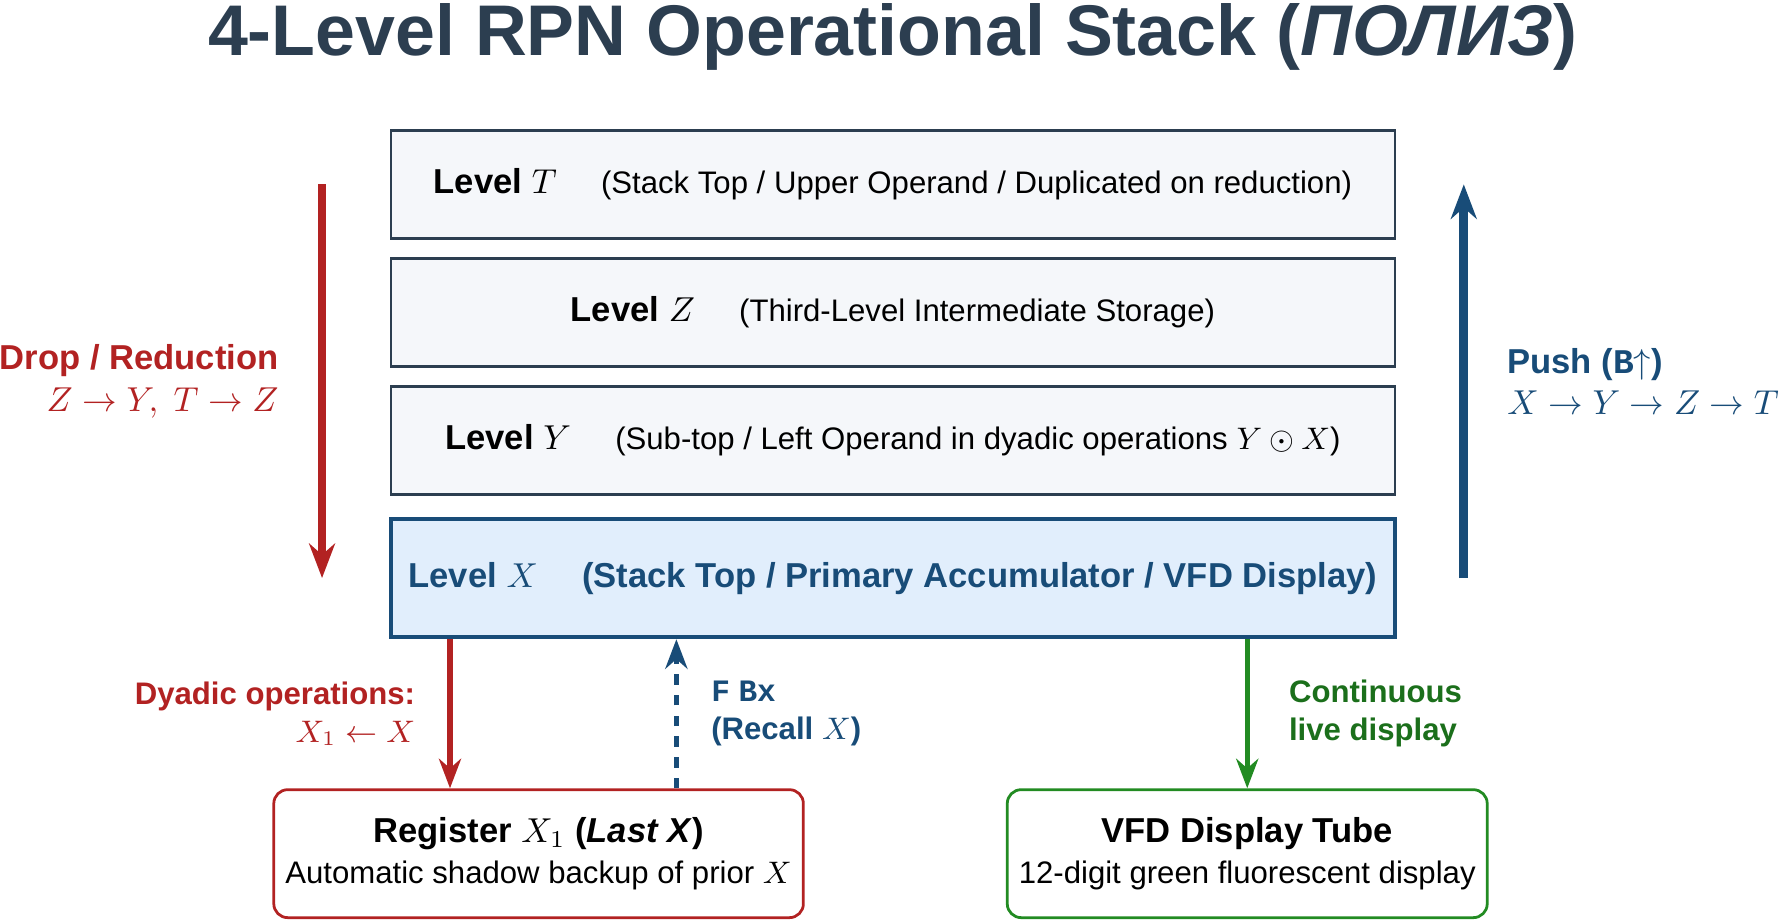
\includegraphics[width=0.92\textwidth]{figures/esquema_pila_en.png}
    \caption{4-Level RPN Operational Stack (\textit{ПОЛИЗ}) Architecture, shadow register $X_1$, and VFD display.}
    \label{fig:pila_en}
\end{figure}

\subsubsection{Stack Register Definitions}
\begin{enumerate}
    \item \textbf{Register $X$ (\textit{Регистр X}):} Stack top (\textit{Вершина стека}). This is the only register continuously reflected on the VFD. It serves as the primary accumulator for all monadic operations and the target for dyadic results.
    \item \textbf{Register $Y$ (\textit{Регистр Y}):} Sub-top. Holds the left operand (first operand) in binary operations: $Y \odot X$.
    \item \textbf{Register $Z$ (\textit{Регистр Z}):} Third-level intermediate storage.
    \item \textbf{Register $T$ (\textit{Регистр T}):} Fourth level of the stack.
    \item \textbf{Register $X_1$ (\textit{Регистр $X_1$ / Предыдущий результат}):} Shadow backup register (\textit{Last X}). Automatically captures the previous contents of $X$ immediately prior to executing any binary arithmetic operation or transcendent function. Restorable into $X$ using the key sequence \texttt{F} \texttt{Bx} (\textit{Восстановление X}).
\end{enumerate}

\subsection{Stack State Dynamics and Transition Matrices}

\subsubsection{A. Data Entry and Duplication: \texorpdfstring{\texttt{В$\uparrow$}}{В-Enter} (\textit{Ввод в стек} / Enter / Push)}
Pressing \texttt{В$\uparrow$} pushes all stack levels upward:
\[
\begin{pmatrix} X \\ Y \\ Z \\ T \end{pmatrix} \xrightarrow{\mathbf{B\uparrow}} \begin{pmatrix} X \\ X \\ Y \\ Z \end{pmatrix}
\]
The value in $X$ is copied to $Y$. The previous value of $T$ is dropped. The register $X$ is preserved, ready to receive incoming digits without overwriting $Y$.

\subsubsection{B. Operand Swap: \texorpdfstring{\texttt{$\leftrightarrow$}}{Swap} (\textit{Обмен X и Y} / Swap)}
Exchanges the contents of the stack top ($X$) and sub-top ($Y$) without altering $Z$ and $T$:
\[
\begin{pmatrix} X \\ Y \\ Z \\ T \end{pmatrix} \xrightarrow{\mathbf{\leftrightarrow}} \begin{pmatrix} Y \\ X \\ Z \\ T \end{pmatrix}
\]

\subsubsection{C. Downward Circular Rotation: \texorpdfstring{\texttt{F} $\circlearrowright$}{F Roll Down} (\textit{Кольцевое перемещение} / Roll Down)}
Cyclically rotates the four stack levels downward:
\[
\begin{pmatrix} X \\ Y \\ Z \\ T \end{pmatrix} \xrightarrow{\mathbf{F\ \circlearrowright}} \begin{pmatrix} Y \\ Z \\ T \\ X \end{pmatrix}
\]
Performing four consecutive rotations (\texttt{F} $\circlearrowright$ $\times 4$) restores the stack precisely to its initial state.

\subsubsection{D. Clear Accumulator: \texttt{Сх} (\textit{Сброс X} / Clear X)}
Clears the active mantissa in $X$ to zero without modifying depth or data in $Y$, $Z$, and $T$:
\[
\begin{pmatrix} X \\ Y \\ Z \\ T \end{pmatrix} \xrightarrow{\mathbf{Cx}} \begin{pmatrix} 0 \\ Y \\ Z \\ T \end{pmatrix}
\]

\subsubsection{E. Dyadic Arithmetic Reduction \texorpdfstring{($+$, $-$, $\times$, $\div$)}{(+, -, *, /)}}
In binary operations where $Y$ is the left-hand operand and $X$ is the right-hand operand ($Y \odot X$):
\begin{enumerate}
    \item The right operand $X$ is stored into the shadow backup register $X_1$ ($X_1 \leftarrow X$).
    \item The evaluated result $Y \odot X$ is written to $X$.
    \item Level $Z$ drops to $Y$ ($Y \leftarrow Z$).
    \item Level $T$ drops to $Z$ ($Z \leftarrow T$).
    \item Level $T$ \textbf{duplicates its value} ($T \leftarrow T$), a distinctive characteristic of PMOS RPN hardware architectures.
\end{enumerate}
\[
\begin{pmatrix} X \\ Y \\ Z \\ T \end{pmatrix} \xrightarrow{\mathbf{+,\ -,\ \times,\ \div}} \begin{pmatrix} Y \odot X \\ Z \\ T \\ T \end{pmatrix}, \qquad X_1 \leftarrow X
\]

\subsubsection{F. Hardware Subroutine Return Stack (\textit{Стек возврата})}
The K145IK1302 core integrates a \textbf{dedicated 5-level LIFO hardware return stack}:
\begin{itemize}
    \item Each subroutine call (\texttt{ПП}) pushes the next sequential address ($PC + 2$) onto the return stack.
    \item Each subroutine return (\texttt{В/О}) pops the top address from the return stack and branches to it.
    \item \textbf{Nesting limit:} Nesting more than 5 levels causes return stack overflow (\textit{circular overwrite}), dropping the oldest return address.
\end{itemize}

\newpage

\section{Memory Map and Registers}

\subsection{Program Memory (\textit{ОЗУ команд})}
\begin{itemize}
    \item \textbf{Total Capacity:} 98 program steps.
    \item \textbf{Address Space:} 2-digit linear decimal addressing from \texttt{00} to \texttt{97}.
    \item \textbf{Instruction Format:} 1 byte per step. Branch instructions taking immediate addresses span two contiguous steps:
    \begin{itemize}
        \item Step $N$: Branch opcode (e.g., \texttt{51} for unconditional jump \texttt{БП}).
        \item Step $N+1$: 2-digit decimal target address (e.g., \texttt{25}).
    \end{itemize}
\end{itemize}

\subsubsection{Operating Modes}
\begin{enumerate}
    \item \textbf{Automatic / Run Mode (\textit{АВТ} / \texttt{F ABT} or \textit{Р} switch):}
    Executes program steps sequentially at full clock speed upon pressing \texttt{С/П} (\textit{Старт/Пуск}).
    \item \textbf{Programming / Edit Mode (\textit{ПРГ} / \texttt{F ПРГ} or \textit{ПРГ} switch):}
    Allows direct reading and writing of program RAM. The VFD adopts the canonical format:
    \[
    \mathbf{AA \quad CC}
    \]
    Where $\mathbf{AA}$ represents the active program address (\texttt{00} to \texttt{97}) and $\mathbf{CC}$ is the opcode byte stored at that address. The keys \texttt{ШГ $\rightarrow$} and \texttt{ШГ $\leftarrow$} step forward and backward through memory.
\end{enumerate}

\subsection{Addressable Data Registers (\textit{Адресуемые регистры})}
The machine features \textbf{14 non-volatile static/dynamic data registers} while powered:
\[
RG0, RG1, RG2, RG3, RG4, RG5, RG6, RG7, RG8, RG9, RGa, RGb, RGc, RGd
\]
Each register stores a full floating-point decimal word (8-digit mantissa and 2-digit signed exponent).

\begin{center}
\small
\begin{tabular}{ccp{7.2cm}p{4.6cm}}
\toprule
\textbf{Register} & \textbf{Key} & \textbf{Behavior in Indirect Mode (\texttt{K})} & \textbf{Common Architectural Use} \\
\midrule
$RG0$ & \texttt{0}       & Auto-decrement by 1 ($RG0 \leftarrow RG0 - 1$) & Loop counter / Downward pointer \\
$RG1$ & \texttt{1}       & Auto-decrement by 1 ($RG1 \leftarrow RG1 - 1$) & Loop counter / Downward pointer \\
$RG2$ & \texttt{2}       & Auto-decrement by 1 ($RG2 \leftarrow RG2 - 1$) & Loop counter / Downward pointer \\
$RG3$ & \texttt{3}       & Auto-decrement by 1 ($RG3 \leftarrow RG3 - 1$) & Loop counter / Downward pointer \\
\midrule
$RG4$ & \texttt{4}       & Auto-increment by 1 ($RG4 \leftarrow RG4 + 1$) & Upward array/memory pointer \\
$RG5$ & \texttt{5}       & Auto-increment by 1 ($RG5 \leftarrow RG5 + 1$) & Upward array/memory pointer \\
$RG6$ & \texttt{6}       & Auto-increment by 1 ($RG6 \leftarrow RG6 + 1$) & Upward array/memory pointer \\
\midrule
$RG7$ & \texttt{7}       & No auto-modification ($RG7 \leftarrow RG7$) & General-purpose data register \\
$RG8$ & \texttt{8}       & No auto-modification ($RG8 \leftarrow RG8$) & General-purpose data register \\
$RG9$ & \texttt{9}       & No auto-modification ($RG9 \leftarrow RG9$) & General-purpose data register \\
$RGa$ & \texttt{.} ($a$) & No auto-modification ($RGa \leftarrow RGa$) & General-purpose data register \\
$RGb$ & \texttt{/-/} ($b$)& No auto-modification ($RGb \leftarrow RGb$) & General-purpose data register \\
$RGc$ & \texttt{ВП} ($c$)& No auto-modification ($RGc \leftarrow RGc$) & General-purpose data register \\
$RGd$ & \texttt{Сх} ($d$)& No auto-modification ($RGd \leftarrow RGd$) & General-purpose data register \\
\bottomrule
\end{tabular}
\end{center}

\subsection{Memory Addressing Modes}
\begin{enumerate}
    \item \textbf{Direct Addressing:}
    \begin{itemize}
        \item \textbf{Store into Register:} \texttt{x$\to$П} $[R]$ (\textit{Запись X в регистр}). Copies accumulator $X$ into register $R$ ($0 \le R \le d$). Accumulator $X$ is preserved.
        \item \textbf{Recall from Register:} \texttt{П$\to$x} $[R]$ (\textit{Вызов из регистра в X}). Pushes the operational stack upward and loads register $R$ into $X$.
    \end{itemize}
    \item \textbf{Indirect Addressing (Prefix \texttt{K}):}
    \begin{itemize}
        \item \textbf{Indirect Store:} \texttt{K} \texttt{x$\to$П} $[R]$. Uses the integer portion of register $R$ as the effective target pointer to store $X$.
        \item \textbf{Indirect Recall:} \texttt{K} \texttt{П$\to$x} $[R]$. Uses the integer portion of register $R$ as the source pointer to load data into $X$.
    \end{itemize}
\end{enumerate}

\begin{techbox}{Critical Automatic Pointer Modification Rule}
Prior to executing an indirect transfer or indirect branch with prefix \texttt{K}:
\begin{itemize}
    \item If $R \in \{0, 1, 2, 3\}$: Pointer register $R$ is \textbf{decremented by 1} ($R \leftarrow R - 1$).
    \item If $R \in \{4, 5, 6\}$: Pointer register $R$ is \textbf{incremented by 1} ($R \leftarrow R + 1$).
    \item If $R \in \{7, 8, 9, a, b, c, d\}$: Pointer register $R$ remains \textbf{unmodified}.
\end{itemize}
\end{techbox}

\newpage

\section{Instruction Set Architecture (Opcodes)}

The following catalog provides the complete instruction set of the Elektronika MK-56 transcribed from the factory manual (\textbf{Table 4 - Таблица 4}).

\subsection{Pseudo-Hexadecimal VFD Display Conventions}
The K145IK1302 microcontroller encodes 4-bit nibbles (\texttt{0x0} to \texttt{0xF}) on 7-segment displays according to Soviet design standards:
\begin{center}
\begin{tabular}{ccp{8.5cm}}
\toprule
\textbf{Hex Nibble} & \textbf{VFD Glyph} & \textbf{Significance / Illuminated Segments} \\
\midrule
\texttt{0x0} -- \texttt{0x9} & \texttt{0} -- \texttt{9} & Standard decimal digits \\
\texttt{0xA} (10) & \texttt{-} & Middle horizontal segment (dash) \\
\texttt{0xB} (11) & \texttt{L} & Lower vertical and bottom horizontal segments (capital L) \\
\texttt{0xC} (12) & \texttt{C} & Top, upper/lower left, and bottom segments (capital C) \\
\texttt{0xD} (13) & \texttt{Г} & Cyrillic Gamma (top and upper left segments) \\
\texttt{0xE} (14) & \texttt{E} & Standard capital E \\
\texttt{0xF} (15) & \textit{blank} & Digit unlit (blank space) \\
\bottomrule
\end{tabular}
\end{center}

\begin{figure}[htbp]
    \centering
    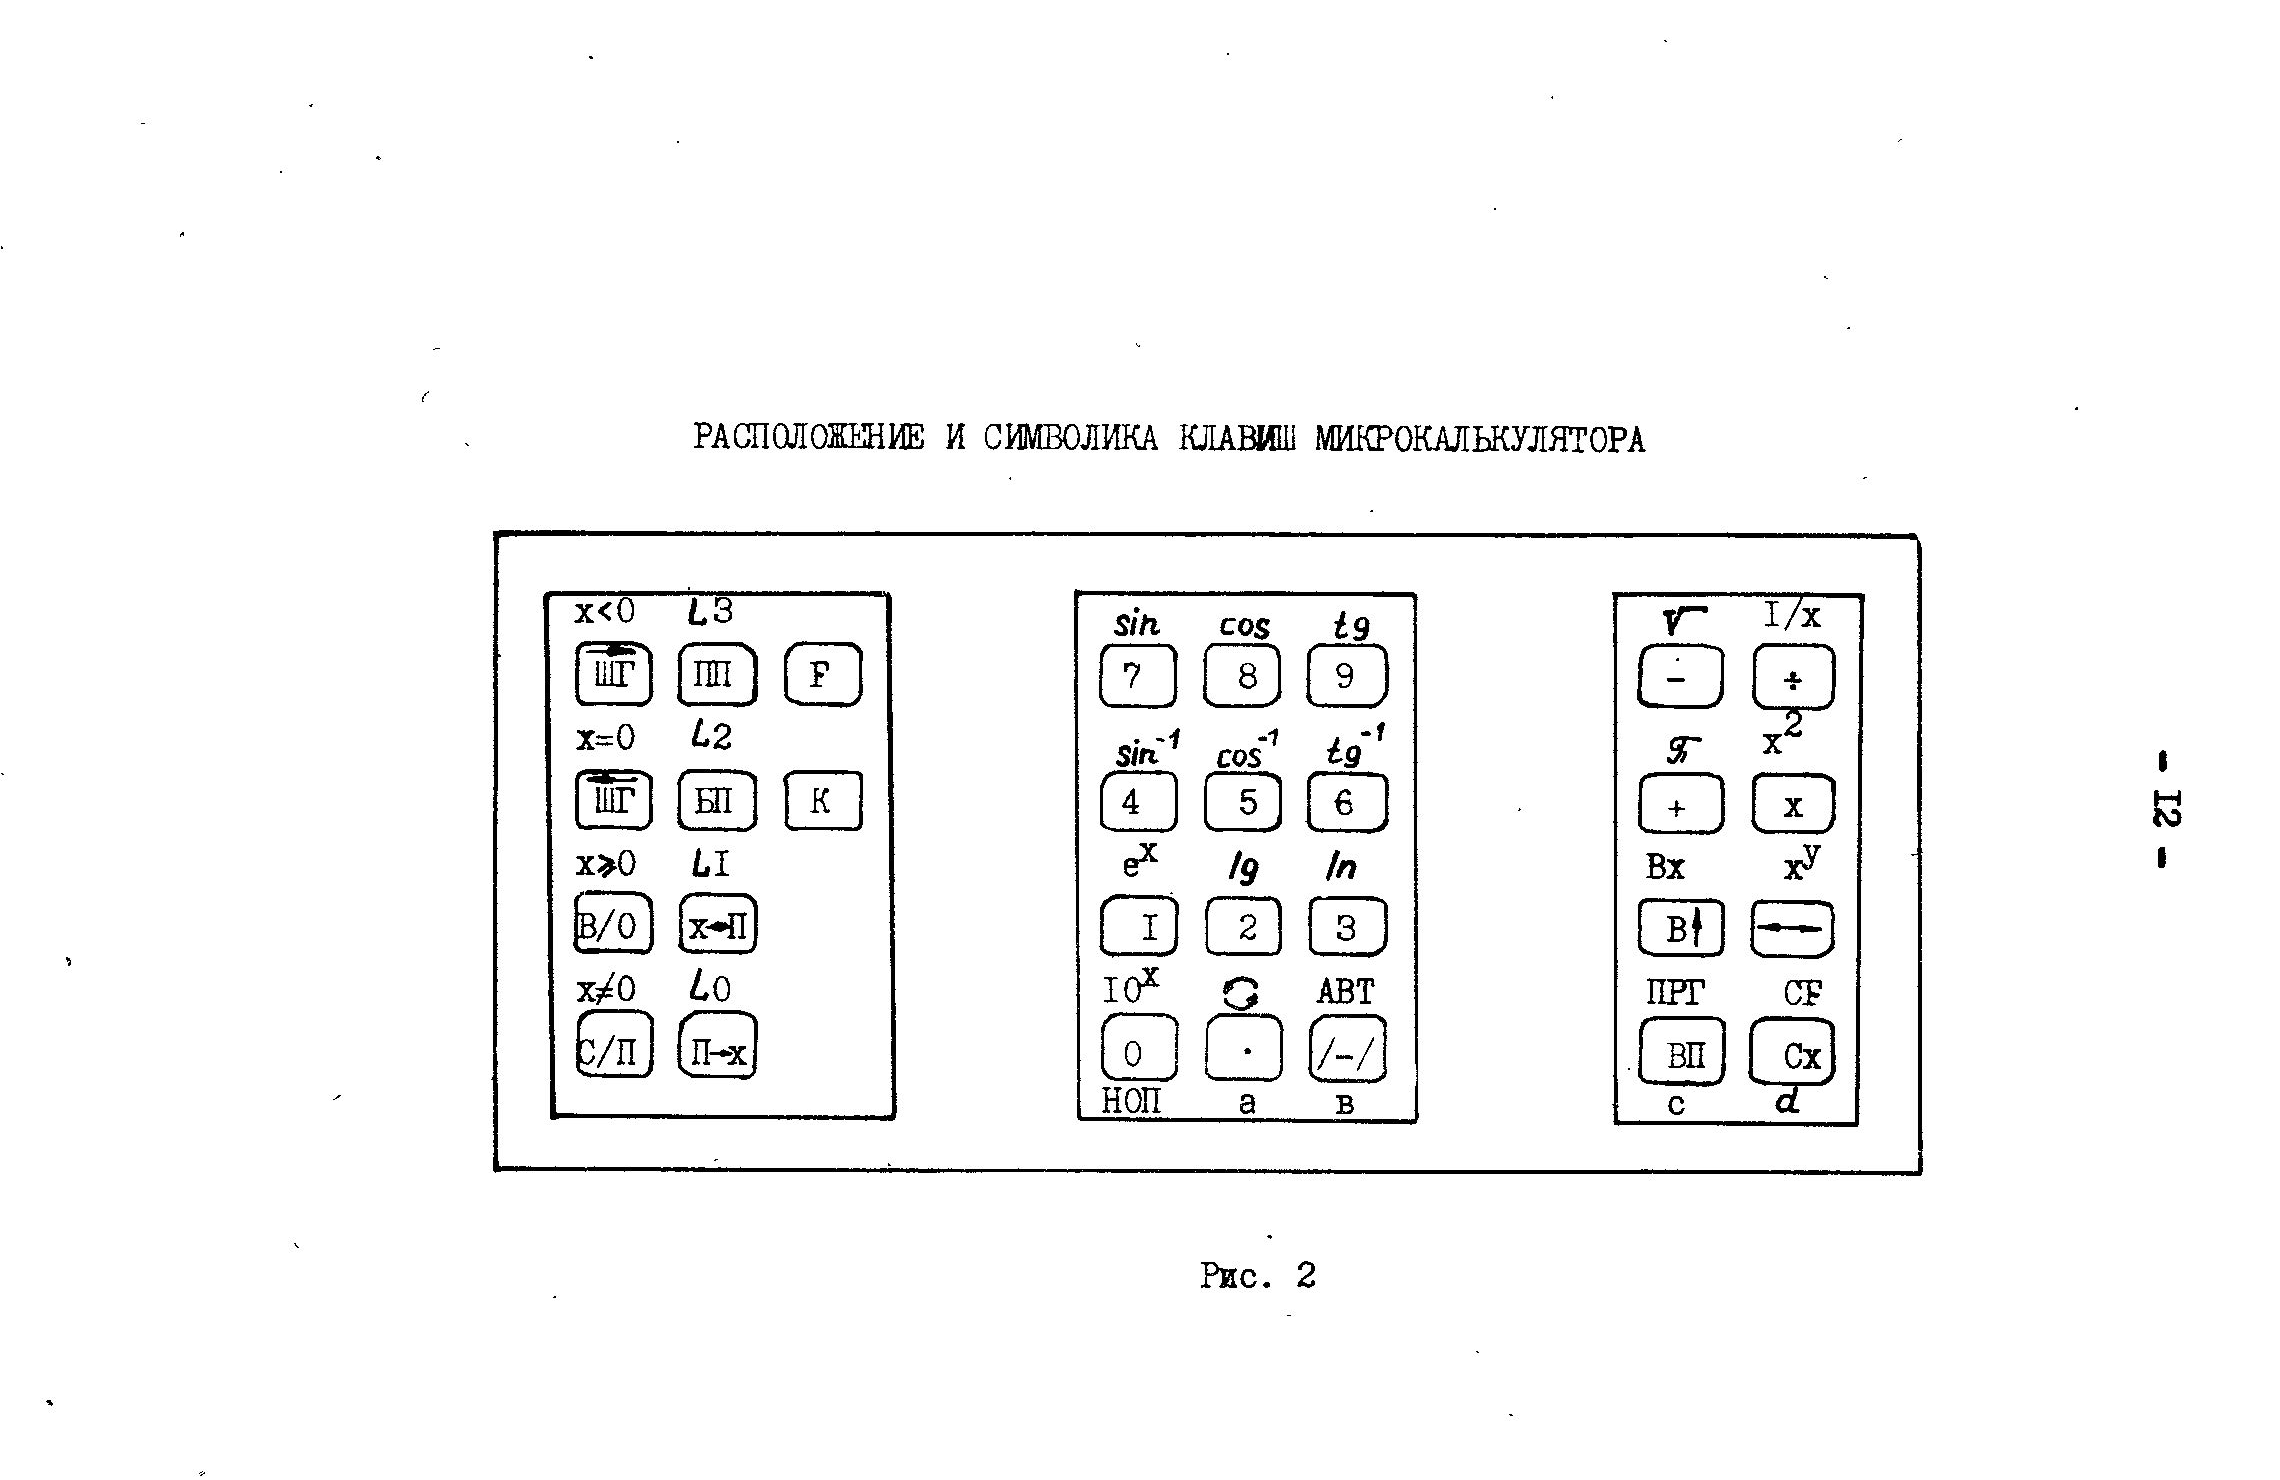
\includegraphics[width=0.90\textwidth]{figures/fig2_teclado_mk56.png}
    \caption{Physical Keyboard Layout and Key Symbols of the Elektronika MK-56 (Figure 2 from the official USSR factory manual).}
    \label{fig:teclado_mk56_en}
\end{figure}

\subsection{Official Instruction Set Table (Таблица 4)}

{\small
\setlength{\tabcolsep}{4pt}
\begin{longtable}{p{2.2cm}p{3.0cm}>{\centering\arraybackslash}p{1.0cm}>{\centering\arraybackslash}p{1.2cm}p{7.3cm}}
\toprule
\textbf{Key (Cyrillic)} & \textbf{English Name} & \textbf{VFD} & \textbf{Hex} & \textbf{Formal Semantics \& Stack Effect} \\
\midrule
\endfirsthead
\toprule
\textbf{Key (Cyrillic)} & \textbf{English Name} & \textbf{VFD} & \textbf{Hex} & \textbf{Formal Semantics \& Stack Effect} \\
\midrule
\endhead
\bottomrule
\endfoot
\texttt{0} & Zero & \texttt{00} & \texttt{0x00} & Loads literal digit 0 into accumulator $X$ \\
\texttt{1} & One & \texttt{01} & \texttt{0x01} & Loads literal digit 1 into accumulator $X$ \\
\texttt{2} & Two & \texttt{02} & \texttt{0x02} & Loads literal digit 2 into accumulator $X$ \\
\texttt{3} & Three & \texttt{03} & \texttt{0x03} & Loads literal digit 3 into accumulator $X$ \\
\texttt{4} & Four & \texttt{04} & \texttt{0x04} & Loads literal digit 4 into accumulator $X$ \\
\texttt{5} & Five & \texttt{05} & \texttt{0x05} & Loads literal digit 5 into accumulator $X$ \\
\texttt{6} & Six & \texttt{06} & \texttt{0x06} & Loads literal digit 6 into accumulator $X$ \\
\texttt{7} & Seven & \texttt{07} & \texttt{0x07} & Loads literal digit 7 into accumulator $X$ \\
\texttt{8} & Eight & \texttt{08} & \texttt{0x08} & Loads literal digit 8 into accumulator $X$ \\
\texttt{9} & Nine & \texttt{09} & \texttt{0x09} & Loads literal digit 9 into accumulator $X$ \\
\texttt{.} & Decimal Point & \texttt{0-} & \texttt{0x0A} & Decimal point separator for active mantissa \\
\texttt{/-/} & Change Sign & \texttt{0L} & \texttt{0x0B} & Inverts sign of accumulator: $X \leftarrow -X$ \\
\texttt{ВП} & Enter Exponent & \texttt{0C} & \texttt{0x0C} & Switches to scientific exponent entry ($EE$) \\
\texttt{Сх} & Clear X & \texttt{0Г} & \texttt{0x0D} & Clears accumulator ($X \leftarrow 0$); stack unchanged \\
\texttt{В$\uparrow$} & Enter / Push & \texttt{0E} & \texttt{0x0E} & Push: $X \to Y, Y \to Z, Z \to T$; preserves $X$ \\
\midrule
\texttt{+} & Addition & \texttt{10} & \texttt{0x10} & $X \leftarrow Y + X;\; Z \to Y;\; T \to Z;\; X_1 \leftarrow X$ \\
\texttt{-} & Subtraction & \texttt{11} & \texttt{0x11} & $X \leftarrow Y - X;\; Z \to Y;\; T \to Z;\; X_1 \leftarrow X$ \\
\texttt{$\times$} & Multiplication & \texttt{12} & \texttt{0x12} & $X \leftarrow Y \times X;\; Z \to Y;\; T \to Z;\; X_1 \leftarrow X$ \\
\texttt{$\div$} & Division & \texttt{13} & \texttt{0x13} & $X \leftarrow Y / X;\; Z \to Y;\; T \to Z;\; X_1 \leftarrow X$ ($X \ne 0$) \\
\texttt{$\leftrightarrow$} & Swap X-Y & \texttt{14} & \texttt{0x14} & Swap: $X \leftrightarrow Y$; levels $Z$ and $T$ unaffected \\
\texttt{F 10\textasciicircum x} & Ten to the Power X & \texttt{15} & \texttt{0x15} & $X \leftarrow 10^X;\; X_1 \leftarrow X$ \\
\texttt{F e\textasciicircum x} & Exponential & \texttt{16} & \texttt{0x16} & $X \leftarrow e^X;\; X_1 \leftarrow X$ \\
\texttt{F lg} & Common Log (Base 10) & \texttt{17} & \texttt{0x17} & $X \leftarrow \log_{10}(X);\; X_1 \leftarrow X$ ($X > 0$) \\
\texttt{F ln} & Natural Log (Base e) & \texttt{18} & \texttt{0x18} & $X \leftarrow \ln(X);\; X_1 \leftarrow X$ ($X > 0$) \\
\texttt{F arcsin} & Arc Sine & \texttt{19} & \texttt{0x19} & $X \leftarrow \arcsin(X);\; X_1 \leftarrow X$ ($|X| \le 1$) \\
\texttt{F arccos} & Arc Cosine & \texttt{1-} & \texttt{0x1A} & $X \leftarrow \arccos(X);\; X_1 \leftarrow X$ ($|X| \le 1$) \\
\texttt{F arctg} & Arc Tangent & \texttt{1L} & \texttt{0x1B} & $X \leftarrow \arctan(X);\; X_1 \leftarrow X$ \\
\texttt{F sin} & Sine & \texttt{1C} & \texttt{0x1C} & $X \leftarrow \sin(X)$; angular mode per toggle switch \\
\texttt{F cos} & Cosine & \texttt{1Г} & \texttt{0x1D} & $X \leftarrow \cos(X)$; angular mode per toggle switch \\
\texttt{F tg} & Tangent & \texttt{1E} & \texttt{0x1E} & $X \leftarrow \tan(X)$; angular mode per toggle switch \\
\midrule
\texttt{F $\pi$} & Constant Pi & \texttt{20} & \texttt{0x20} & Loads $\pi \approx 3.1415926$ into $X$; pushes stack \\
\texttt{F $\sqrt{x}$} & Square Root & \texttt{21} & \texttt{0x21} & $X \leftarrow \sqrt{X};\; X_1 \leftarrow X$ ($X \ge 0$) \\
\texttt{F x\textasciicircum 2} & Square & \texttt{22} & \texttt{0x22} & $X \leftarrow X^2;\; X_1 \leftarrow X$ \\
\texttt{F 1/x} & Reciprocal & \texttt{23} & \texttt{0x23} & $X \leftarrow 1/X;\; X_1 \leftarrow X$ ($X \ne 0$) \\
\texttt{F x\textasciicircum y} & Arbitrary Power & \texttt{24} & \texttt{0x24} & $X \leftarrow Y^X;\; Z \to Y;\; T \to Z;\; X_1 \leftarrow X$ \\
\midrule
\texttt{x$\to$П 0} & Store to RG0 & \texttt{40} & \texttt{0x40} & $RG0 \leftarrow X$; accumulator $X$ preserved \\
\texttt{x$\to$П 1} & Store to RG1 & \texttt{41} & \texttt{0x41} & $RG1 \leftarrow X$; accumulator $X$ preserved \\
\texttt{x$\to$П 2} & Store to RG2 & \texttt{42} & \texttt{0x42} & $RG2 \leftarrow X$; accumulator $X$ preserved \\
\texttt{x$\to$П 3} & Store to RG3 & \texttt{43} & \texttt{0x43} & $RG3 \leftarrow X$; accumulator $X$ preserved \\
\texttt{x$\to$П 4} & Store to RG4 & \texttt{44} & \texttt{0x44} & $RG4 \leftarrow X$; accumulator $X$ preserved \\
\texttt{x$\to$П 5} & Store to RG5 & \texttt{45} & \texttt{0x45} & $RG5 \leftarrow X$; accumulator $X$ preserved \\
\texttt{x$\to$П 6} & Store to RG6 & \texttt{46} & \texttt{0x46} & $RG6 \leftarrow X$; accumulator $X$ preserved \\
\texttt{x$\to$П 7} & Store to RG7 & \texttt{47} & \texttt{0x47} & $RG7 \leftarrow X$; accumulator $X$ preserved \\
\texttt{x$\to$П 8} & Store to RG8 & \texttt{48} & \texttt{0x48} & $RG8 \leftarrow X$; accumulator $X$ preserved \\
\texttt{x$\to$П 9} & Store to RG9 & \texttt{49} & \texttt{0x49} & $RG9 \leftarrow X$; accumulator $X$ preserved \\
\texttt{x$\to$П a} & Store to RGa & \texttt{4-} & \texttt{0x4A} & $RGa \leftarrow X$; accumulator $X$ preserved \\
\texttt{x$\to$П b} & Store to RGb & \texttt{4L} & \texttt{0x4B} & $RGb \leftarrow X$; accumulator $X$ preserved \\
\texttt{x$\to$П c} & Store to RGc & \texttt{4C} & \texttt{0x4C} & $RGc \leftarrow X$; accumulator $X$ preserved \\
\texttt{x$\to$П d} & Store to RGd & \texttt{4Г} & \texttt{0x4D} & $RGd \leftarrow X$; accumulator $X$ preserved \\
\midrule
\texttt{С/П} & Start / Stop & \texttt{50} & \texttt{0x50} & Halts or initiates automatic execution \\
\texttt{БП} & Unconditional Jump & \texttt{51} & \texttt{0x51} & Direct jump: $PC \leftarrow \text{immediate byte } (N+1)$ \\
\texttt{В/О} & Return / Reset & \texttt{52} & \texttt{0x52} & Return from subroutine (pop stack) or $PC \leftarrow \texttt{00}$ \\
\texttt{ПП} & Call Subroutine & \texttt{53} & \texttt{0x53} & Push $PC+2$ to return stack; $PC \leftarrow \text{byte } (N+1)$ \\
\texttt{K НОП} & No Operation (NOP) & \texttt{54} & \texttt{0x54} & No Operation; advances $PC \leftarrow PC+1$ \\
\texttt{F x$\ne$0} & Branch if $X \ne 0$ & \texttt{57} & \texttt{0x57} & \textbf{Inverted:} If $X = 0 \Rightarrow$ jump to $N+1$; If $X \ne 0 \Rightarrow PC+2$ \\
\texttt{F L2} & Loop Counter RG2 & \texttt{58} & \texttt{0x58} & $RG2 \leftarrow RG2-1$; If $RG2 \ne 0 \Rightarrow$ jump; If 0 $\Rightarrow PC+2$ \\
\texttt{F x$\ge$0} & Branch if $X \ge 0$ & \texttt{59} & \texttt{0x59} & \textbf{Inverted:} If $X < 0 \Rightarrow$ jump to $N+1$; If $X \ge 0 \Rightarrow PC+2$ \\
\texttt{F L3} & Loop Counter RG3 & \texttt{5-} & \texttt{0x5A} & $RG3 \leftarrow RG3-1$; If $RG3 \ne 0 \Rightarrow$ jump; If 0 $\Rightarrow PC+2$ \\
\texttt{F L1} & Loop Counter RG1 & \texttt{5L} & \texttt{0x5B} & $RG1 \leftarrow RG1-1$; If $RG1 \ne 0 \Rightarrow$ jump; If 0 $\Rightarrow PC+2$ \\
\texttt{F x$<$0} & Branch if $X < 0$ & \texttt{5C} & \texttt{0x5C} & \textbf{Inverted:} If $X \ge 0 \Rightarrow$ jump to $N+1$; If $X < 0 \Rightarrow PC+2$ \\
\texttt{F L0} & Loop Counter RG0 & \texttt{5Г} & \texttt{0x5D} & $RG0 \leftarrow RG0-1$; If $RG0 \ne 0 \Rightarrow$ jump; If 0 $\Rightarrow PC+2$ \\
\texttt{F x$=$0} & Branch if $X = 0$ & \texttt{5E} & \texttt{0x5E} & \textbf{Inverted:} If $X \ne 0 \Rightarrow$ jump to $N+1$; If $X = 0 \Rightarrow PC+2$ \\
\midrule
\texttt{П$\to$x 0} & Recall from RG0 & \texttt{60} & \texttt{0x60} & Loads $RG0$ into $X$; pushes operational stack \\
\texttt{П$\to$x 1} & Recall from RG1 & \texttt{61} & \texttt{0x61} & Loads $RG1$ into $X$; pushes operational stack \\
\texttt{П$\to$x 2} & Recall from RG2 & \texttt{62} & \texttt{0x62} & Loads $RG2$ into $X$; pushes operational stack \\
\texttt{П$\to$x 3} & Recall from RG3 & \texttt{63} & \texttt{0x63} & Loads $RG3$ into $X$; pushes operational stack \\
\texttt{П$\to$x 4} & Recall from RG4 & \texttt{64} & \texttt{0x64} & Loads $RG4$ into $X$; pushes operational stack \\
\texttt{П$\to$x 5} & Recall from RG5 & \texttt{65} & \texttt{0x65} & Loads $RG5$ into $X$; pushes operational stack \\
\texttt{П$\to$x 6} & Recall from RG6 & \texttt{66} & \texttt{0x66} & Loads $RG6$ into $X$; pushes operational stack \\
\texttt{П$\to$x 7} & Recall from RG7 & \texttt{67} & \texttt{0x67} & Loads $RG7$ into $X$; pushes operational stack \\
\texttt{П$\to$x 8} & Recall from RG8 & \texttt{68} & \texttt{0x68} & Loads $RG8$ into $X$; pushes operational stack \\
\texttt{П$\to$x 9} & Recall from RG9 & \texttt{69} & \texttt{0x69} & Loads $RG9$ into $X$; pushes operational stack \\
\texttt{П$\to$x a} & Recall from RGa & \texttt{6-} & \texttt{0x6A} & Loads $RGa$ into $X$; pushes operational stack \\
\texttt{П$\to$x b} & Recall from RGb & \texttt{6L} & \texttt{0x6B} & Loads $RGb$ into $X$; pushes operational stack \\
\texttt{П$\to$x c} & Recall from RGc & \texttt{6C} & \texttt{0x6C} & Loads $RGc$ into $X$; pushes operational stack \\
\texttt{П$\to$x d} & Recall from RGd & \texttt{6Г} & \texttt{0x6D} & Loads $RGd$ into $X$; pushes operational stack \\
\midrule
\texttt{K x$\ne$0 [R]} & Indirect Branch $X \ne 0$ & \texttt{70}--\texttt{7Г} & \texttt{0x70}--\texttt{0x7D} & Test $X \ne 0$ via pointer in $RG0..RGd$ \\
\texttt{K БП [R]} & Indirect Uncond. Jump & \texttt{80}--\texttt{8Г} & \texttt{0x80}--\texttt{0x8D} & Indirect jump to target address in $R$ \\
\texttt{K x$\ge$0 [R]} & Indirect Branch $X \ge 0$ & \texttt{90}--\texttt{9Г} & \texttt{0x90}--\texttt{0x9D} & Test $X \ge 0$ via pointer in $RG0..RGd$ \\
\texttt{K ПП [R]} & Indirect Subroutine & \texttt{-0}--\texttt{-Г} & \texttt{0xA0}--\texttt{0xAD} & Indirect call to address in $RG0..RGd$ \\
\texttt{K x$\to$П [R]} & Indirect Store & \texttt{L0}--\texttt{LГ} & \texttt{0xB0}--\texttt{0xBD} & Stores $X$ into register pointed by $R$ \\
\texttt{K x$<$0 [R]} & Indirect Branch $X < 0$ & \texttt{C0}--\texttt{CГ} & \texttt{0xC0}--\texttt{0xCD} & Test $X < 0$ via pointer in $RG0..RGd$ \\
\texttt{K П$\to$x [R]} & Indirect Recall & \texttt{Г0}--\texttt{ГГ} & \texttt{0xD0}--\texttt{0xDD} & Loads into $X$ from register pointed by $R$ \\
\texttt{K x$=$0 [R]} & Indirect Branch $X = 0$ & \texttt{E0}--\texttt{EГ} & \texttt{0xE0}--\texttt{0xED} & Test $X = 0$ via pointer in $RG0..RGd$ \\
\bottomrule
\end{longtable}
}

\newpage

\section{Control Flow and Branching}

\subsection{Direct Unconditional Jump: \texttt{БП} (\textit{Безусловный переход})}
Encoded across 2 contiguous program memory steps:
\begin{itemize}
    \item \textbf{Step $N$:} Opcode \texttt{51} (\texttt{БП}).
    \item \textbf{Step $N+1$:} Target 2-digit decimal address ($00$ to $97$).
\end{itemize}
The sequencer assigns the immediate destination to the program counter: $PC \leftarrow \text{Target}$.

\subsection{Subroutine Call and Return: \texttt{ПП} and \texttt{В/О}}
\begin{itemize}
    \item \textbf{Subroutine Call (\texttt{ПП} -- \textit{Переход к подпрограмме}):}
    2-step instruction: Opcode \texttt{53} followed by destination address. Pushes $PC + 2$ onto the 5-level hardware LIFO return stack, then branches: $PC \leftarrow \text{Address}$.
    \item \textbf{Subroutine Return (\texttt{В/О} -- \textit{Возврат / Отмена}):}
    1-step instruction: Opcode \texttt{52}. Pops the top address from the hardware return stack and transfers execution there.
    \item \textbf{Root Level Behavior:} If executed outside a subroutine (return stack empty), \texttt{В/О} resets the program counter to zero ($PC \leftarrow 00$).
\end{itemize}

\subsection{Inverted Conditional Branch Mechanics}

\begin{warnbox}{Architectural Quirk of the B3-34 / MK-56 Family: Inverted Branching}
In contrast to standard computing architectures (such as x86 or ARM) where a jump occurs when a condition is met:
\begin{center}
\textbf{The Elektronika MK-56 BRANCHES ONLY IF THE TEST CONDITION IS FALSE (\textit{условие НЕ выполняется}).}
\end{center}
If the test condition evaluates to \textbf{TRUE}, the processor \textbf{ignores the branch address} at $N+1$ and proceeds sequentially to the next instruction ($PC \leftarrow N + 2$).
\end{warnbox}

\begin{figure}[htbp]
    \centering
    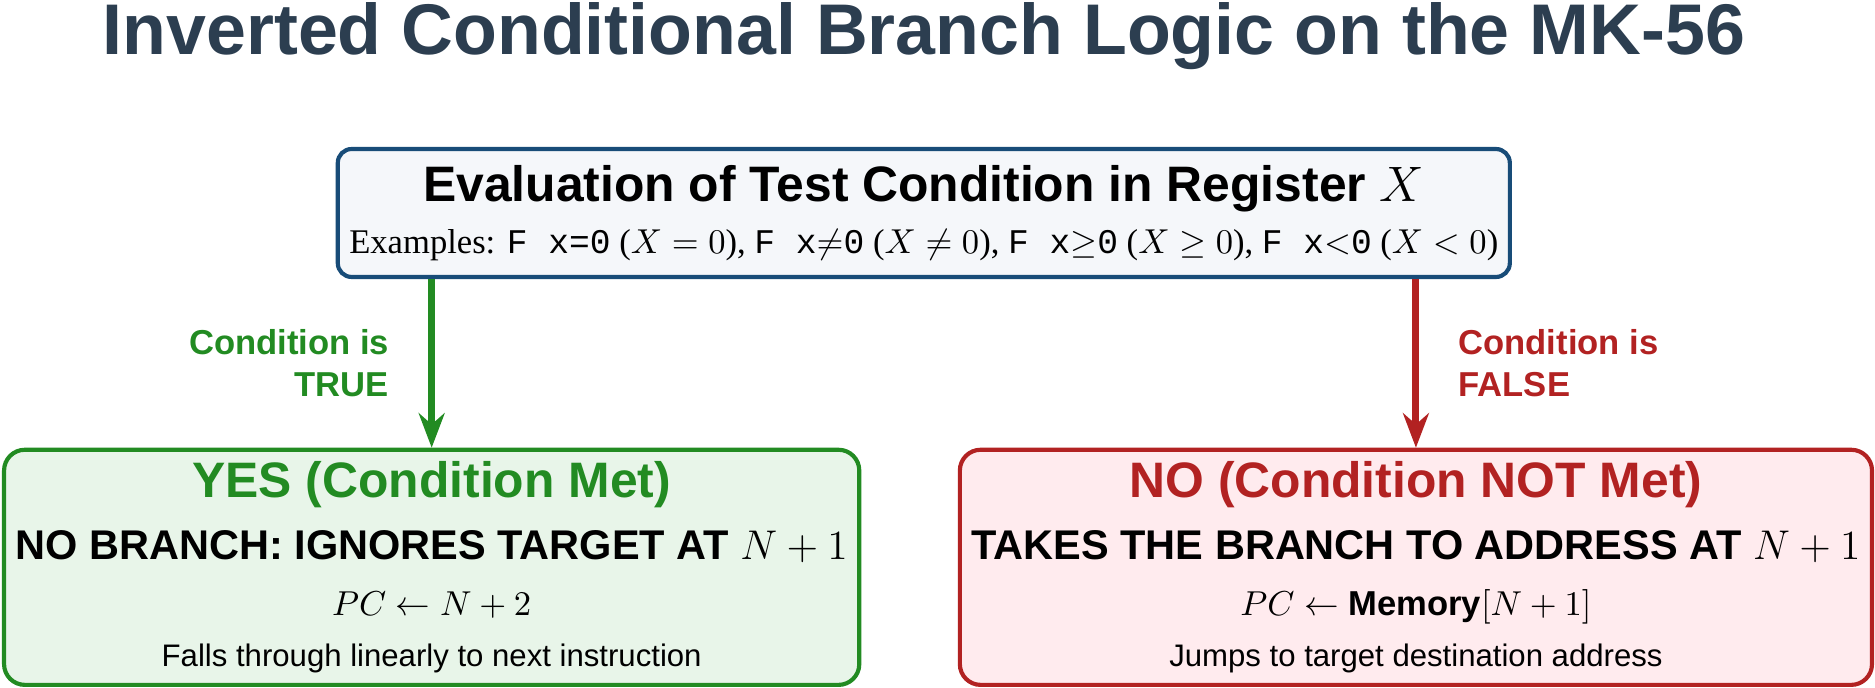
\includegraphics[width=0.95\textwidth]{figures/esquema_salto_en.png}
    \caption{Inverted Conditional Branch Decision Flowchart on the Elektronika MK-56.}
    \label{fig:salto_en}
\end{figure}

\subsubsection{Formal Conditional Branch Specifications}
\begin{enumerate}
    \item \texttt{F x=0} (\textbf{Opcode \texttt{5E}}):
    \begin{itemize}
        \item If $X \ne 0$ (False): \textbf{Branches} to address at $N+1$.
        \item If $X = 0$ (True): \textbf{Does not branch}; advances to $N+2$.
    \end{itemize}
    \item \texttt{F x$\ne$0} (\textbf{Opcode \texttt{57}}):
    \begin{itemize}
        \item If $X = 0$ (False): \textbf{Branches} to address at $N+1$.
        \item If $X \ne 0$ (True): \textbf{Does not branch}; advances to $N+2$.
    \end{itemize}
    \item \texttt{F x$\ge$0} (\textbf{Opcode \texttt{59}}):
    \begin{itemize}
        \item If $X < 0$ (False): \textbf{Branches} to address at $N+1$.
        \item If $X \ge 0$ (True): \textbf{Does not branch}; advances to $N+2$.
    \end{itemize}
    \item \texttt{F x$<$0} (\textbf{Opcode \texttt{5C}}):
    \begin{itemize}
        \item If $X \ge 0$ (False): \textbf{Branches} to address at $N+1$.
        \item If $X < 0$ (True): \textbf{Does not branch}; advances to $N+2$.
    \end{itemize}
\end{enumerate}

\subsubsection{Compiler Code Generation Pattern for Conditional Constructs}
To compile a high-level construct such as:
\begin{center}
\texttt{if (X == 0) \{ ThenBlock \} else \{ ElseBlock \}}
\end{center}
\begin{center}
\begin{tcolorbox}[colback=codebg,colframe=darkslate,width=0.95\textwidth]
\begin{verbatim}
; At step N:
F x=0           ; Opcode 5E: Branch to else if X != 0
label_else      ; Address of Else block (step N+1)
; ThenBlock begins here (executes linearly if X == 0)
...
БП              ; Opcode 51: Unconditional jump over Else block
label_end       ; Exit address
label_else:
; ElseBlock begins here (reached if X != 0)
...
label_end:
\end{verbatim}
\end{tcolorbox}
\end{center}

\subsection{Hardware Loop Counters: \texttt{F L0}, \texttt{F L1}, \texttt{F L2}, \texttt{F L3}}
Specialized 2-step loop control instructions providing automated decrement and termination tests:
\begin{itemize}
    \item \textbf{Loop Opcodes:}
    \texttt{F L0} $\to$ \texttt{5Г} ($RG0$); \quad
    \texttt{F L1} $\to$ \texttt{5L} ($RG1$); \quad
    \texttt{F L2} $\to$ \texttt{58} ($RG2$); \quad
    \texttt{F L3} $\to$ \texttt{5-} ($RG3$).
    \item \textbf{Execution Mechanics:}
    \begin{enumerate}
        \item Decrements the integer unit of the designated register:
        \[
        RGk \leftarrow RGk - 1 \qquad (k \in \{0, 1, 2, 3\})
        \]
        \item Evaluates the resulting value:
        \begin{itemize}
            \item \textbf{If $RGk \ne 0$:} The loop continues; jumps to address at $N+1$ ($PC \leftarrow \text{Target}$).
            \item \textbf{If $RGk = 0$:} The loop terminates; continues linearly to step $N+2$ ($PC \leftarrow N + 2$).
        \end{itemize}
    \end{enumerate}
\end{itemize}

\begin{figure}[htbp]
    \centering
    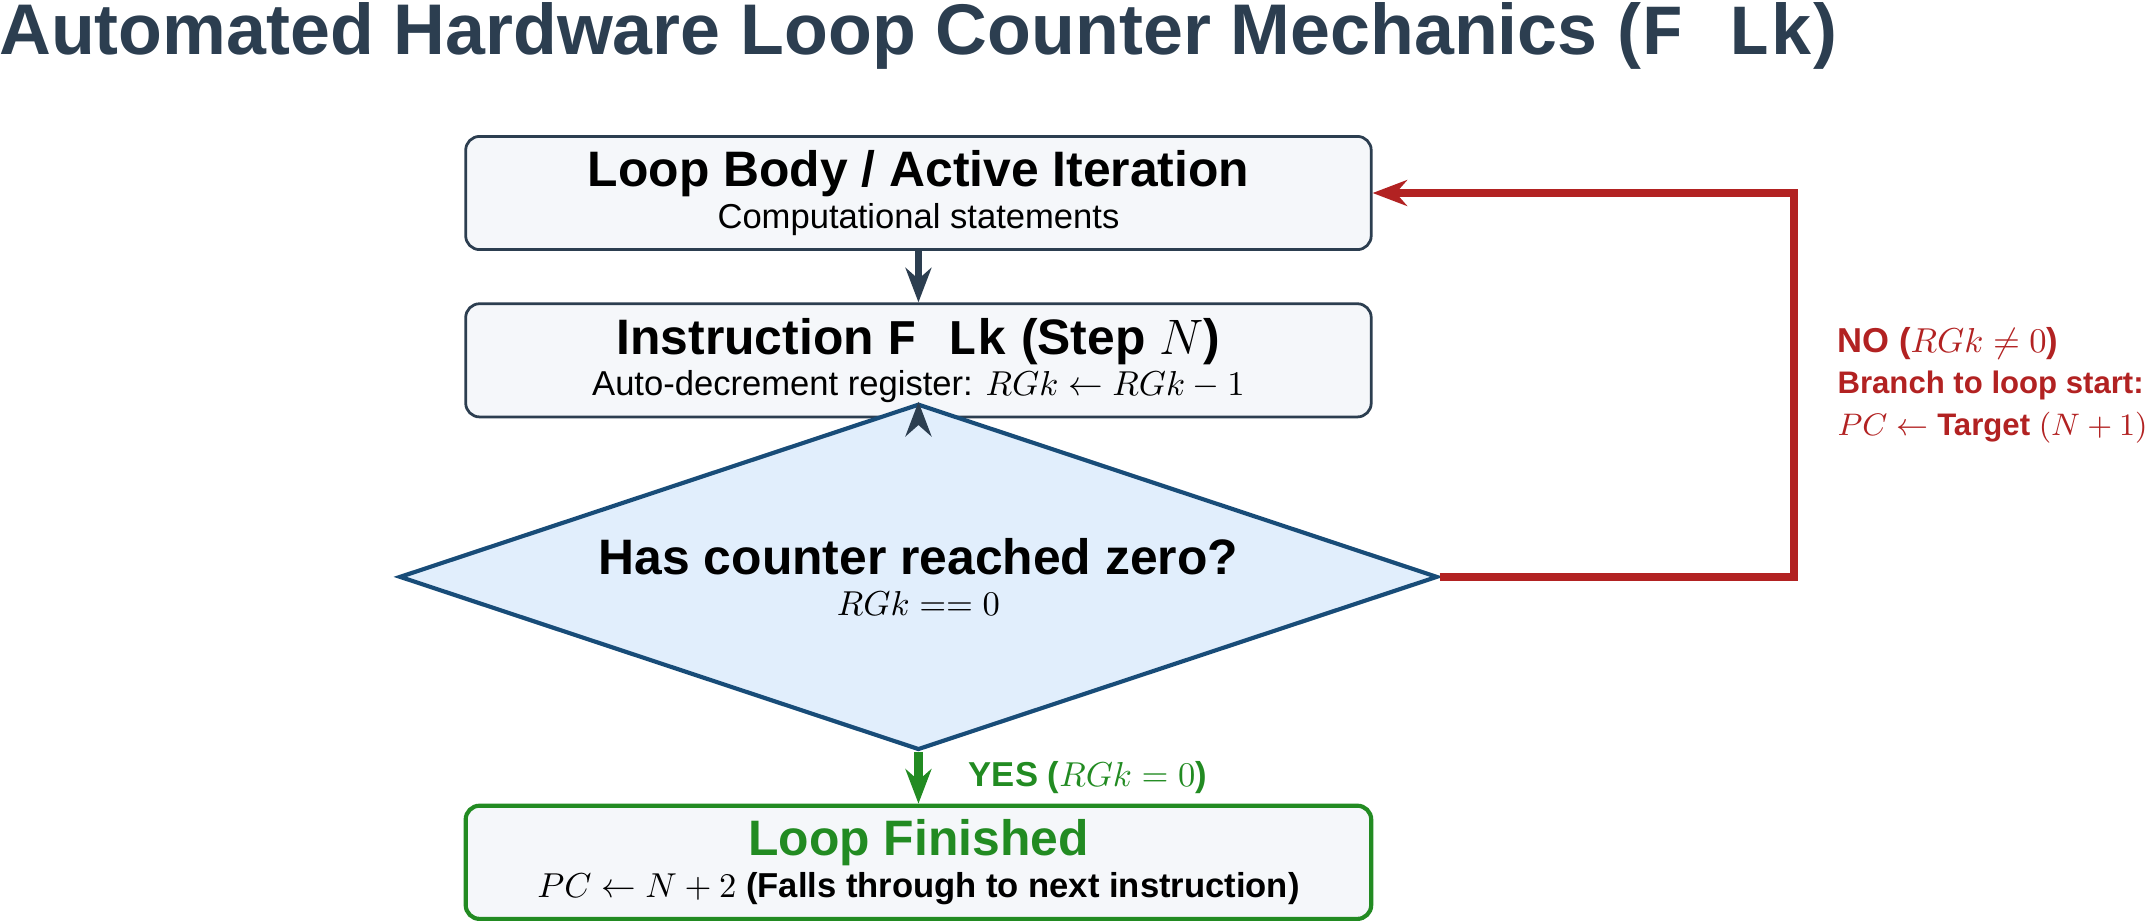
\includegraphics[width=0.88\textwidth]{figures/esquema_bucle_en.png}
    \caption{Control Cycle Flowchart for Hardware Automated Loop Counters (\texttt{F Lk}).}
    \label{fig:bucle_en}
\end{figure}

\subsection{Indirect Branching and Dynamic Dispatch}
The MK-56 supports indirect unconditional branches, indirect subroutine calls, and indirect conditional tests where the target address is \textbf{dynamically loaded from a data register}. These instructions occupy \textbf{a single program byte}:
\begin{itemize}
    \item \textbf{Indirect Unconditional Jump:} \texttt{K БП [R]} (Opcodes \texttt{80} to \texttt{8Г}). Modifies $R$ (if $R \le 6$) and branches to the integer address in $R$.
    \item \textbf{Indirect Subroutine Call:} \texttt{K ПП [R]} (Opcodes \texttt{-0} to \texttt{-Г}). Pushes return address ($PC + 1$) to return stack, modifies $R$, and branches.
    \item \textbf{Indirect Conditional Branches:} \texttt{K x=0}, \texttt{K x$\ne$0}, \texttt{K x$\ge$0}, \texttt{K x$<$0}. Evaluates $X$; if condition is false, modifies $R$ and branches to address in $R$. If true, advances to $PC + 1$ without modifying $R$.
\end{itemize}

\newpage

\section{Architectural Specification Summary for Compiler Engineers}

\begin{center}
\renewcommand{\arraystretch}{1.2}
\setlength{\tabcolsep}{5pt}
\begin{tabular}{p{5.8cm}p{9.8cm}}
\toprule
\textbf{Architectural Parameter} & \textbf{Technical Specification} \\
\midrule
\textbf{Execution Model} & Pure Reverse Polish Notation (RPN) with top-of-stack accumulator ($X$) \\
\textbf{Operational Stack Depth} & 4 hardware levels: $X, Y, Z, T$ \\
\textbf{Backup Register} & 1 automatic shadow register: $X_1$ (\textit{Last X}) \\
\textbf{Subroutine Call Stack Depth} & 5 dedicated hardware LIFO levels \\
\textbf{Code Memory (RAM)} & 98 addressable program steps (\texttt{00} to \texttt{97}) \\
\textbf{Data Registers} & 14 floating-point registers ($RG0..RG9, RGa..RGd$) \\
\textbf{Opcode Length} & 1 byte per instruction; branch address in subsequent byte \\
\textbf{Conditional Branch Logic} & \textbf{Inverted:} branches when condition is FALSE; falls through when TRUE \\
\textbf{Auto-decrementing Registers} & $RG0, RG1, RG2, RG3$ (decremented by 1 when accessed via \texttt{K}) \\
\textbf{Auto-incrementing Registers} & $RG4, RG5, RG6$ (incremented by 1 when accessed via \texttt{K}) \\
\textbf{Hardware Loop Counters} & 4 dedicated instructions: \texttt{F L0}, \texttt{F L1}, \texttt{F L2}, \texttt{F L3} \\
\textbf{VFD Display Glyphs} & Standard \texttt{0..9}; \texttt{A}$\to$\texttt{-}, \texttt{B}$\to$\texttt{L}, \texttt{C}$\to$\texttt{C}, \texttt{D}$\to$\texttt{Г}, \texttt{E}$\to$\texttt{E}, \texttt{F}$\to$\textit{blank} \\
\bottomrule
\end{tabular}
\end{center}

\subsection{Practical IR Code Generation Guidelines}
When constructing a compiler code generator targeting MK-56 bytecode:
\begin{enumerate}
    \item \textbf{Static Stack Depth Tracking:} The compiler must compute stack depth at each IR node. Because the operational stack is limited to 4 levels, expressions requiring more than 4 concurrent intermediate values must spill temporary registers (typically $RG7..RGd$) using \texttt{x$\to$П} and restore them via \texttt{П$\to$x}.
    \item \textbf{Conditional Inversion Mapping:} When emitting conditional jumps:
    \[
    \text{Emit } \mathtt{F\ x=0} \implies \text{Branch to failure label if } X \ne 0
    \]
    \[
    \text{Emit } \mathtt{F\ x\neq0} \implies \text{Branch to failure label if } X = 0
    \]
    \[
    \text{Emit } \mathtt{F\ x\ge0} \implies \text{Branch to failure label if } X < 0
    \]
    \[
    \text{Emit } \mathtt{F\ x<0} \implies \text{Branch to failure label if } X \ge 0
    \]
    \item \textbf{Loop Optimization:} For bounded loops with iteration counts known at runtime in the range $1..99$, allocate the loop counter into one of $RG0..RG3$ and close the loop using \texttt{F Lk}, eliminating separate decrement and branch instructions.
\end{enumerate}

\end{document}
